\documentclass[a4paper,twocolumn]{article}
\usepackage[utf8]{inputenc}
\usepackage{booktabs}
\usepackage{xcolor}
\usepackage{listings}
\usepackage{microtype}
\usepackage{syntax}
\usepackage{amsmath}
\usepackage[backend=biber]{biblatex}
\usepackage{tikz}
\usepackage{tikz-qtree}
\usetikzlibrary{shapes,patterns,positioning}
\usepackage{minted}
\usepackage[
  colorlinks,
  linkcolor={red!40!black},
  citecolor={blue!60!black},
  urlcolor={blue!60!black}
]{hyperref}

\addbibresource{references.bib}

\title{Reverse Polish Notation:\\A Gentle Introduction to Stack Machines}
\author{Patrick M. Elsen <pelsen@xfbs.net>}
\date{\input{_tag}}

% make this a reproducible build
\pdfvariable suppressoptionalinfo \numexpr32+64+512\relax

\begin{document}
\maketitle
\tableofcontents

\section*{Introduction}

Stack Machines are a good way to get acquainted with computing concepts because they are very accessible and typically simpler to work with than register machines. Reverse Polish Notation is not only historically interesting due to its use in a lot of early calculators, but also in practise due to the simplicity with which they can be implemented.

This article gives the reader an introduction to both by providing examples and easy challenges that can be completed. It assumes some background in computer science, knowledge of using command-line utilities and some programming knowledge in C++.

Following the example of  poc||gtfo, this \textsc{pdf} is also a valid \textsc{zip} file, containing code discussed here and the source code to this very article. Use the \verb|unzip| command to extract this information.

\begin{verbatim}
$ unzip rpn.pdf
\end{verbatim}
Find the latest version of this article at \href{https://github.com/xfbs/rpn}{github.com/xfbs/rpn} and feel free to redistribute as you like.

\section{Overview}

Reverse Polish Notation is a way to write down equations without needing to use brackets or precedence rules. This greatly simplifies parsing. For this reason, reverse polish notation has been quite popular with Hewlett-Packard calculators\cite{website:hprpn}\footnote{In fact, all of the desktop and hand-held calculators produced in the 70ies and 80ies by  Hewlett-Packard used Reverse-Polish Notation.}.

Take a simple mathematical equation with the four primitive operators — addition, subtraction, multiplication and division.

\begin{equation}\label{eqn:simpleeqn}
  \frac{(1 + 2) * (7 - 3)}{2 * 6}
\end{equation}

The rules dictate the order in which the operations should be executed, and brackets can be used to override those rules where necessary. For example, in the expression $1 + 2 * 7 - 3$, the multiplication of 2 and 7 would be evaluated first, and only then would the additions and multiplications be evaluated, because multiplication has a higher precedence.

This precedence can be overridden by using parentheses, to force addition to be evaluated before multiplicatiom. The \textsc{pedmas} mnemonic is a good way to remember the order of precedence: \emph{parentheses, exponentiation, division, multiplication, addition, subtraction}. 

In our mind, we can parse this equation into a tree that represents the order of operations.

\begin{center}
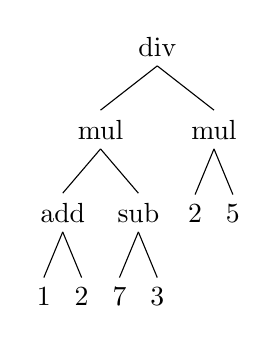
\begin{tikzpicture}
\Tree [.div [.mul [.add 1 2 ] [.sub 7 3 ] ] [.mul 2 5 ] ]
\end{tikzpicture}
\end{center}

In this tree notation, operations are performed bottom-up. The addition of 1 and 2 and the subtraction of 3 from 7 are performed first, the results of that multiplied, et cetera.


If we think about trees, then the way we write down equations normally is called the \emph{inorder} notation, meaning that we write down the nodes in the order in which they appear in the tree, from left to right.

\begin{center}
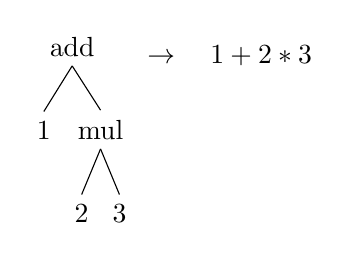
\begin{tikzpicture}
\Tree [.add 1 [.mul 2 3 ] ];
\node (abc) at (2,0) {$\to \quad 1 + 2 * 3$};
\end{tikzpicture}
\end{center}

This is somewhat intuitive for humans to parse because there is higher locality. But this format also has some issues with it, in that it needs to be parsed and precedence to be applied before it can be executed. Imagine parsing an equation like $1 + 2 * 3$. You have to parse the \emph{entire} equation first, because there might always be a higher-precedented operation after.

When using reverse polish notation, you simply rearrange the equations to something called the \emph{postorder}. This means that the child nodes are put first, and then the parent nodes.

\begin{center}
\begin{tikzpicture}
\Tree [.mul [.add 1 2 ] 3 ];
\node (abc) at (2.5,0) {$\to\quad1\quad2\quad+\quad3\quad*$};
\end{tikzpicture}
\end{center}

The advantage of this is immediately obvious: it becomes possible to execute this without parsing the entire thing. The way this is executed is by using a stack. 

When executing this, imagine going through a stream of the tokens $[1, 2, +, 3, *]$. Execution starts at the first token, a 1. This is data, and thus it is placed on the stack. Then the next token is encountered, a 2. This, again, is data and thus placed on the stack. Thus far, the stack contain $[1, 2]$ on it. Next, $+$ is encountered, which is an operation that takes two operands. Thus, the last two items are popped from the stack, added, and the result pushed back on it. Thus, at this point, the stack contains only $[3]$. Visually, this means that we have simplified the expression tree as such:

\begin{center}
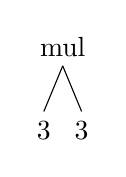
\begin{tikzpicture}
\Tree [.mul 3 3 ];
\end{tikzpicture}
\end{center}

Next, we encounter the token 3, which again, is data and is pushed on the stack. The stack now contains $[3, 3]$, where the first three is the result of the addition, and the second three is data. Lastly, a $*$ is encountered, which is a multiplication operation, which takes two items off the stack, multiplies them, and pushes the result, a 9, back onto the stack.

\begin{table}[h!]
\centering
\caption{Executing a simple RPN}\label{tlb:simplerpn}
\begin{tabular}{@{}clp{5cm}@{}}
\toprule
Token & Stack & Comment\\
\midrule
1 & 1 & Push 1 onto the stack.\\
2 & 1, 2 & Push 2 onto the stack.\\
$+$ & 3 & Adds last two items on stack.\\
3 & 3, 3 & Push 3 onto the stack.\\
$*$ & 9 & Multiplies last two items on stack.\\
\bottomrule  
\end{tabular}
\end{table}

Table \ref{tlb:simplerpn} illustrates this process in a more organised way. With this knowledge, Equation \ref{eqn:simpleeqn} can be transformed into reverse polish notation rather easily:

\begin{equation}
1\quad2\quad+\quad7\quad3\quad-\quad*\quad2\quad6\quad*\quad/  
\end{equation}

In a sense, reverse polish notation forms a sort of bridge between the world of mathematics and the world of computer science, because reverse polish notation is both a way to represent equations and a kind of instruction stream that can be processed by a virtual stack machine to evaluate it.

\subsection*{Exercises}

\begin{enumerate}
  \item Convert the following equations to \textsc{rpn}.
  \begin{align*}
    &{1 * 2}^{9 - 2} &
    \frac{9 - 2 - 3 + 4}{5 * 2}
  \end{align*}
  
  \item Calculate the result of the following \textsc{rpn} equation.
  \begin{equation*}
    355\quad113\quad/\quad2\quad*\quad30\quad11\quad6\quad/\quad+\quad*
  \end{equation*}
\end{enumerate}

\section{Interpreting Reverse Polish Notation}

As explained previously, reverse polish notation is very simple to evaluate. This can be demonstrated by writing an interpreter for it that supports only some simple mathematical operations.

Let us define a simple syntax for a reverse polish notation that only supports numbers and four simple math operators. To make it as simple to parse as possible, a space has to be between every one of the tokens.

\setlength{\grammarindent}{4em}
\begin{grammar}

<program> ::= <token> <space> <program>
              \alt <token>

<token> ::= <number> | <operator>

<number> ::= <digit> <number> | <digit>

<digit> ::= ‘0’ | ‘1’ | ‘2’ | ‘3’ | ‘4’ | ‘5’
\alt ‘6’ | ‘7’ | ‘8’ | ‘9’

<space> ::= ‘ ’ 

\end{grammar}

An example program that follows this grammar might look like in equation (2).
\begin{equation}
1\quad2\quad+\quad7\quad3\quad-\quad*\quad2\quad6\quad*\quad/  
\end{equation}

The C++ standard library offers facilities for splitting a string into space-separated tokens.

\begin{minted}{cpp}
#include <iostream>
#include <sstream>
#include <string>

int main() {
    std::string program = "1 2 + 7 3 - *";
    std::istringstream iss(program);
    std::string token;

    while(iss >> token) {
        // parse token
    }
}  
\end{minted}

To parse individual tokens, string comparison and number parsing library functions can be used, as every token is either a known operator or number.

\begin{minted}{cpp}
if(tok == "+") {
    return new Add();
} else if(tok == "*") {
    return new Mul();
} else if(tok == "-") {
    return new Sub();
} else if(tok == "/") {
    return new Div();
} else {
    return new Num(std::stod(tok));
}
\end{minted}

Here, the function \verb|std::stod()| is a C++ function to parse a number from a string, and \verb|Add()|, \verb|Mul()|, \verb|Sub()|, \verb|Div()| all subclasses of an abstract Operation class.

To represent the stack, the C++ \verb|std::deque<double>| is a good candidate, because it has efficient pop and push operations, but it also allows index-based access to elements, which is useful for displaying the stack.

With this in mind, the execute functions for the number token can look somewhat like this, simply pushing the number that it was constructed with onto the stack.

\begin{minted}{cpp}
void Num::execute(std::deque<double> &s) {                                                                                                                                                           
    s.push_back(number);                                                                                                                                                                                
}  
\end{minted}

Similarly, the other operations can be implemented, by popping values off the stack and pushing the result back onto it. Here is the addition, implemented by taking the last two numbers off the stack, and pushing the result of the addition back onto it.

\begin{minted}{cpp}
void Add::execute(std::deque<double> &s) {
    double rhs = s.back();
    s.pop_back();
    double lhs = s.back();
    s.pop_back();
    s.push_back(lhs + rhs);
}  
\end{minted}

Like this, a Reverse-Polish Notation interpreter can be crafted in less than 200 lines of code. 

There is working example code for this in the \verb|rpn-calc| folder. After every sequence of tokens, it prints out the entire stack, making examining the state very easy.

\begin{verbatim}
$ make rpn-calc
...
$ ./rpn-calc/build/calc-cli
> 1
1
> 2
1 2
> +
3
> 3 4 -
3 -1
> *
-3
\end{verbatim}
This particular interpreter only supports the four basic math operators, but it is very simple to extend the code to make it support more.

In fact, there are existing reverse polish notation interpreters and compilers that support a lot more. There's even one on your printer right now -- we'll get to that one in a bit.

\subsection*{Exercises}

\begin{enumerate}
  \item Compile the \verb|rpn-calc| tool from the code in this repository. If you don't have the code, you can extract it from this \textsc{pdf} file as documented in the introduction. Run the \verb|calc-cli| tool and try out some expressions like \verb|1 2 +|.

  \item Can you add \verb|^| as exponentiation operator to the interpreter? Hint: create a class named \verb|Exp()|, add an \verb|Exp::execute(...)| method and add it to the parser.
\end{enumerate}

While it's always good fun and educational to implement reverse polish notation interpreters ourselves, it is perhaps more interesting to examine existing implementations that are already sitting on your system. We can take a look at three particular implementations — \textsc{gnu dc}, Adobe PostScript and Forth. If none of these ring any bells, don't worry. 

\section{Math with GNU DC}

There are some utilities sitting on almost every \textsc{unix}-like system\footnote{which is most systems these days, taking macOS, iOS and Android into account} that rarely anyone has ever had the pleasure to interact with directly, and yet they have great power.

Out of those obscure utilities, we will take a look at one of them: \textsc{dc}. It might just be the oldest and yet most universal reverse polish notation interpreter — but I don't have references on that. There is only one place where you might have stumbled across it, and that is StackOverflow Code Golfing. It is definitely an esoteric language\footnote{\url{https://esolangs.org/wiki/Dc}}, which, if you are into that kinda stuff, makes it even more interesting.

 Its name is an acronym for \emph{desktop calculator}, and that is exactly what it does. You can and should pop open the manual page for \verb|dc| to get a bit of information about it, as well as a command reference.

\begin{verbatim}
$ man dc
\end{verbatim}

Unlike our previous little calculator, \textsc{dc} does not require that tokens are separated by spaces. Also, it has a lot more operators (commands), which are all single-letter. 

It looks really quite cryptic, especially because it is character-based. It can do simple addition like we did before. One difference is that it does not implicitly print the stack -- but the \verb|p| command exists to print the stack.

\begin{verbatim}
$ dc -e "1 2 3 + + p"
6
\end{verbatim}

It is not limited to working with numbers — by enclosing it in \verb|[| and \verb|]| square brackets, \textsc{dc} can work with strings of text as well. Thus, an example of printing some text looks like this.

\begin{verbatim}
$ dc -e "[Hello World]p"
Hello World  
\end{verbatim}

It is obvious that \textsc{dc} can do quite a lot more than just adding numbers and printing the result. At this point, we have to leave mathematics a bit behind on this journey, and introduce some programming constructs such as dictionaries and lists that are not typically found in a math context.

Not only can the strings be used for storing text, but also for storing code, which can be executed. Such code can be stored into a register with \verb|sr|, where \verb|r| is a letter denoting which register it is saved to, and run with \verb|x|.

By writing a macro that conditionally calls itself, a loop can be implemented.

\begin{verbatim}
$ dc -e "[p1-d0<r]sr10lrx"
10
9
8
...
1
\end{verbatim}

To explain how this works, we can take it apart. There is a macro, the string \verb|[p-1d0<r]|, prints the current top of the stack, decrements it by 1, and recursively calls itself if the result of that is not smaller than zero. After that, \verb|sr| saves this macro into register \verb|r|. Next 10 is loaded onto the stack, and the macro in \verb|r| executed with \verb|lrx|. In Table \ref{tlb:dcloop}, the instructions are listed and explained.

\begin{table}[!h]
\centering
\caption{Explanation of the \textsc{dc} program.}\label{tlb:dcloop}
\begin{tabular}{@{}lp{5.7cm}@{}}
\toprule
Command & Explanation \\
\midrule
\verb|[| & Start string.\\
\verb|p| & Print top of stack.\\
\verb|1| & Push 1 on stack.\\
\verb|-| & Subtract top of stack from second.\\
\verb|d| & Duplicate top of stack.\\
\verb|0| & Push 0 on stack.\\
\verb|<r| & Execute contents of register r if second top is smaller than top of stack.\\
\verb|]| & End string.\\
\verb|sr| & Store string in register r.\\
\verb|10| & Push 10 to stack.\\
\verb|lr| & Load contents of register r.\\
\verb|x| & Execute top of stack.\\
\bottomrule
\end{tabular}
\end{table}

\subsection*{Exercises}

\begin{enumerate}
  \item Write a \textsc{dc} script that will find the sum of numbers from 1 to 100.
  \item Write a \textsc{dc} script that will find the first number larger than 1000.
\end{enumerate}

\section{PostScript}

PostScript is another one of those things that most people haven't ever heard of or used. But unlike \textsc{dc}, this is something you may very well have used.

Back in the 80ies when Adobe was one of the pioneers of digital printing, they needed some way to send data to printers in an efficient manner.

When you want to print a page, you can render it into a large image and send that off. This is not a particularily great idea, however. If we look at A4, which is the standard paper size you will find in printers, they have a size of 200mm $\times$ 283. Printing is often done at a resolution of 300 or 600 DPI. At this resolution, a whole document would take about 4 GB to be represented.

The idea with PostScript is that instead of rendering a document as an image locally and sending the (potentially large) image to the printer, we can generate a PostScript program that will generate it, and this can be run on the printer itself.

Such a program can be considerably smaller, especially for documents that consist of text and vector drawings.

PostScript is implemented as a stack machine. But unlike our small \textsc{rpn} calculator, it is a fairly powerful programming language, supporting functions, variables, arrays and dictionaries.

It is quite impractical to send off a program to a printer and have it burn polymers onto dead tree carcasses every time a it needs to be run. Therefore, there is a project called \emph{GhostScript}, which is a PostScript interpreter that runs on your local system.

An interactive PostScript prompt can be launched with it by running the \verb|gs| executable.\cite{bluebook1985}

\begin{verbatim}
$ gs -dNODISPLAY
GS> 1 2 add stack
3
\end{verbatim}

Similar to \textsc{dc}, PostScript also supports strings, but they are delimited by parentheses and not brackets. 

\begin{minted}{postscript}
(Hello World\n) print  
\end{minted}

PostScript also supports defining routines. The basic syntax looks like this.

\begin{minted}{postscript}
/name {
  % function body
} def
\end{minted}

Here, \verb|/name| puts the symbol \emph{name} onto the stack. In the braces is code, which is also put on the stack. The call to \verb|def| pops the name and the code off the stack and defines it.

With this knowledge, and a few basic PostScript commands, recursive fibonacci can be implemented.

\begin{minted}{postscript}
/fibonacci {
    % check if these are the first two.
    dup 2 lt

    {   % if so, return 1.
        pop
        1
    } { % otherwise compute sum of
        % fibonacci(n-1) and 
        % fibonacci(n-2)
        dup 2 sub
        fibonacci
        exch 1 sub
        fibonacci
        add
    } ifelse
} def
\end{minted}



\subsection*{Exercises}

\begin{enumerate}
  \item Install GhostScript on your local system (if you are on macOS, it should come preinstalled, otherwise check your package manager) and run the example code in the \verb|postscript| directory.
 
  \item Can you write a function that will compute the largest common multiple of two numbers?
\end{enumerate}

\section{Forth}

After having taken a look at \textsc{dc} and PostScript, which are both interpreted, higher-level languages, we can now look into a slightly different direction and examine another oddity out of the programming languages world, Forth. 

\section{Obscure Code Golfing with 05AB1E}



\section{Generating}

Now that we know what reverse polish notation is (the \emph{postorder} of a tree) and how we can interpret it (by working through a stream of tokens), the last interesting aspect that is left is to find out how we can generate reverse polish notation from regular infix notation. 

We have already discussed the parse tree, and this is exactly how we translate from one format into another.

In the \verb|rpn-gen| folder you will find a parser, written in C++, that will emit reverse polish notation (in a format that \verb|rpn-calc| understands). 

\subsection*{Exercises}

\begin{enumerate}
  \item Can you implement parsing of exponentiation, such that \verb|1 ^ 2| generates \verb|1 2 ^|?
  \item Why does the parser have to parse the entire tree before it can generate \textsc{rpn}?
\end{enumerate}

\section{Conclusion}

Reverse Polish Notation is an interesting format because it is very accessible — having no complex syntax, parsing or precedence rules. This is what makes it interesting for hackers writing their own little custom interpreters or for people new in the field.

We have also seen that it is not 

The disadvantage of \textsc{rpn} is that the code is not as readable.

\printbibliography

\end{document}
